%
%  Simulation BSP
%
%  Created by Johannes Kasberger on 2011-07-15.
\documentclass[a4paper]{article}

\usepackage[utf8]{inputenc}
\usepackage{ngerman}
\usepackage{fullpage}
\usepackage{listings}
\usepackage{ifpdf}
\usepackage[pdftex]{graphicx}

\title{Diskrete Regelung}
\author{Johannes Kasberger\\Markus Klein\\Simon Sperl}

\date{Juli 2011}

\begin{document}

\maketitle

\section{Füllstandsregelung eines Viertanksystems}

Es ist folgender Aufbau gegeben: Vier Tanks sind miteinander durch Röhren verbunden. Ein Motor pumpt Wasser in den ersten Tank und das Wasser fließt im letzten Tank ab. Der Querschnitt der Röhren ist grundsätzlich einstellbar, bleibt jedoch während des Betriebs konstant. Das Ziel ist es, den Füllstand im letzten Tank auf eine gewünschte Höhe zu regeln. Ein kontinuierlicher Regler der diese Aufgabe erfüllt, ist im Buch Modellbildung und Simulation dynamischer Systeme von H.E. Schärf beschrieben. Unsere Aufgabe ist es dieses kontinuierlichen Regler in einen diskreten Regler umzuwandeln. Das Model der Tanks haben wir vom Buch übernommen und in einen Simulink Block gekapselt. 

Der Regler ist im Buch als PID Regler ausgeführt. Um daraus einen diskreten Regler bauen zu können, muss die Übertragungsfunktion diskretisiert werden. Das geschieht mit der Matlab Funktion c2d. Wenn man die Übertragungsfunktion eines idealen Reglers so transformiert, funktioniert der digitale Regler aber nicht richtig. Es muss noch eine parasitäre Zeitkonstante zum kontinuierlichen Regler hinzugefügt werden (somit wird er zum realen PID Regler) und dieser kann dann diskretisiert werden. Diese Rechnung passiert in der Datei \emph{koef.m }. Darin werden auch alle benötigten Konstanten definiert, daher muss diese Datei ausgeführt werden um das Simulink Model lauffähig zu machen. 

Um das Verhalten des diskreten und des kontinuierlichen Reglers vergleichen zu können, haben wir die Zwei gleichzeitig simuliert und die Ergebnisse in einem Plot dargestellt (Abbildung \ref{fig:bsp1}). Der Plot zeigt, dass das Verhalten der zwei Regler gut übereinstimmt. Die Abweichung der Stellgrößen der Regler beträgt maximal 3 und pendelt sonst immer um 0 (ist im mittleren Plot in Abbildung \ref{fig:bsp1}). Der Füllstand im oberen Plot und auch die Stellgrößen im unteren Plot sind weitgehend deckungsgleich.

Der diskrete Regler wurde in zwei Varianten realisiert. Einmal mit dem Simulink Block \emph{Discrete Filter} (in Datei diskre.mdl realisiert). Die Koeffizienten für diesen Filter werden in der Datei koef.m berechnet und hier verwendet. Die andere Variante (in der Datei diskr\_matlab.mdl zu finden) verwendet eine selbst geschriebene Embedded Matlab Function. Darin wird die Matlab Function \emph{filter} verwendet, um die Inputdaten zu filtern. Die Koeffizienten sind die Gleichen wie bei der Simulink Variante (siehe Abbildung \ref{fig:bsp1_code}).

\begin{figure}[ht!]
    \centering
    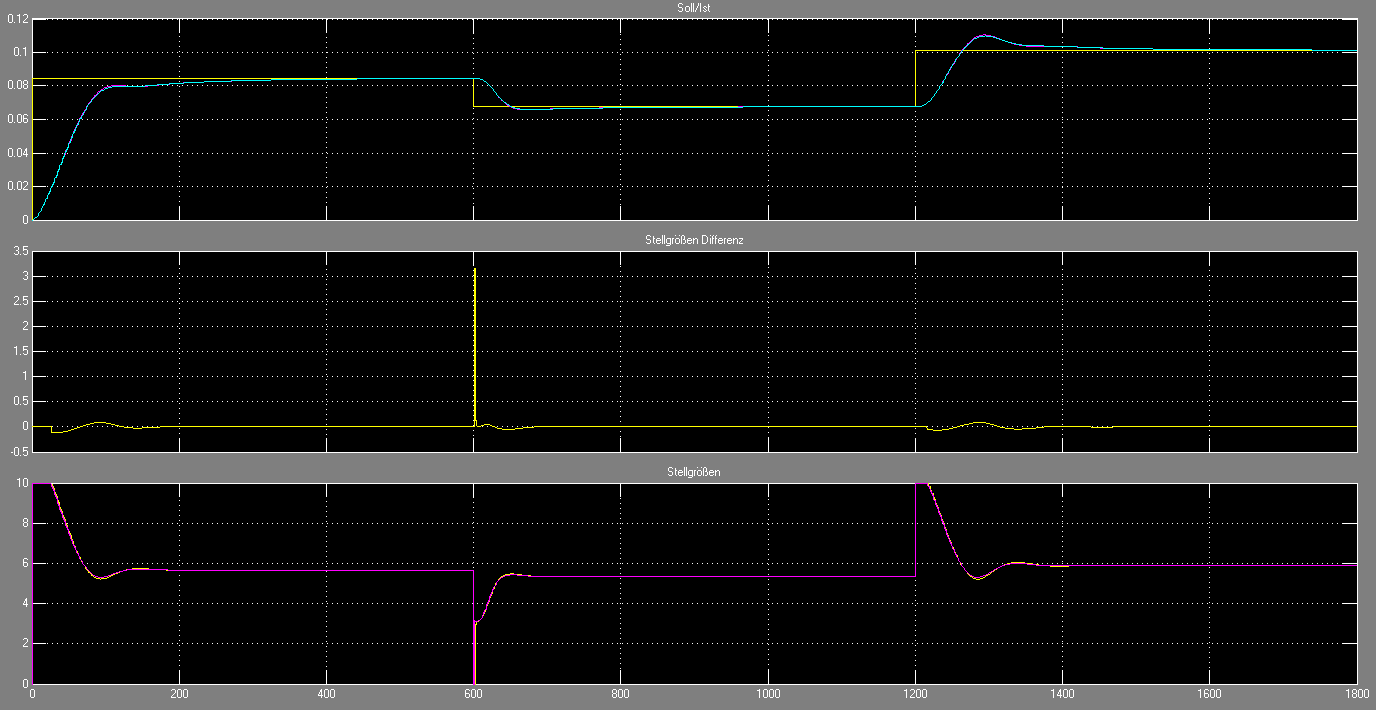
\includegraphics[width=\linewidth]{erg_bsp1.png}
    \caption{Vergleich Kontinuierlicher/Diskreter Regler}
    \label{fig:bsp1}
\end{figure}

\begin{figure}[ht!]
    \centering
    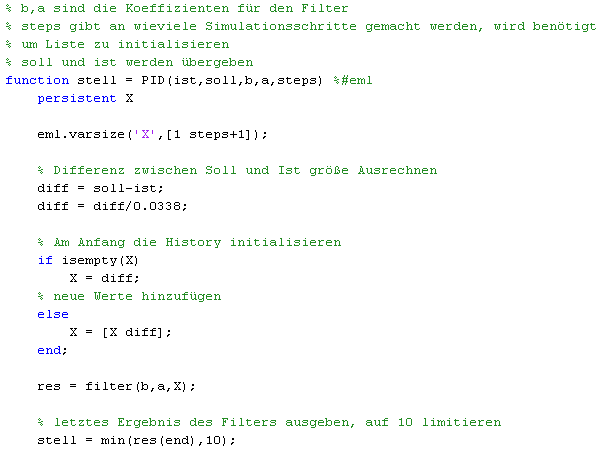
\includegraphics[width=\linewidth]{code_bsp1.png}
    \caption{Code für Realisierung als Matlab Function}
    \label{fig:bsp1_code}
\end{figure}

\section{Aufheizen eines Werkstücks in einem Glühofen}

\section{Fahrradmodell}

Nach einer Unstimmigkeit in der Systemgleichung des Modells haben wir uns für die einheitmäßig korrekte Gleichung nach G. Retschitzegger entschieden.

Um das Modell simulieren zu können, mussten noch eine Vielzahl von anderen Konstanten bestimmt werden. Nach einer Parameterstudie, für die zwei kontinuierliche Regler implementiert wurden, fanden wir die in \emph{koeff.m} gelisteten Parameter als gute Simulationsbasis.



\end{document}
